\documentclass[tikz,border=2pt]{standalone}
\usepackage[T1]{fontenc}
\usepackage[scaled]{helvet}
\renewcommand{\familydefault}{\sfdefault}
\usepackage{tikz}
\usetikzlibrary{external,calc,shapes.callouts,shapes.arrows}
\usetikzlibrary{arrows.meta,patterns,patterns.meta,shapes.arrows}
\usetikzlibrary{decorations.pathreplacing}
\tikzset{>=Latex,
  max width/.style args={#1}{
    execute at begin node={\begin{varwidth}{#1}},
    execute at end node={\end{varwidth}}
  }
}
\usetikzlibrary{shapes}
\usetikzlibrary{external}
\begin{document}
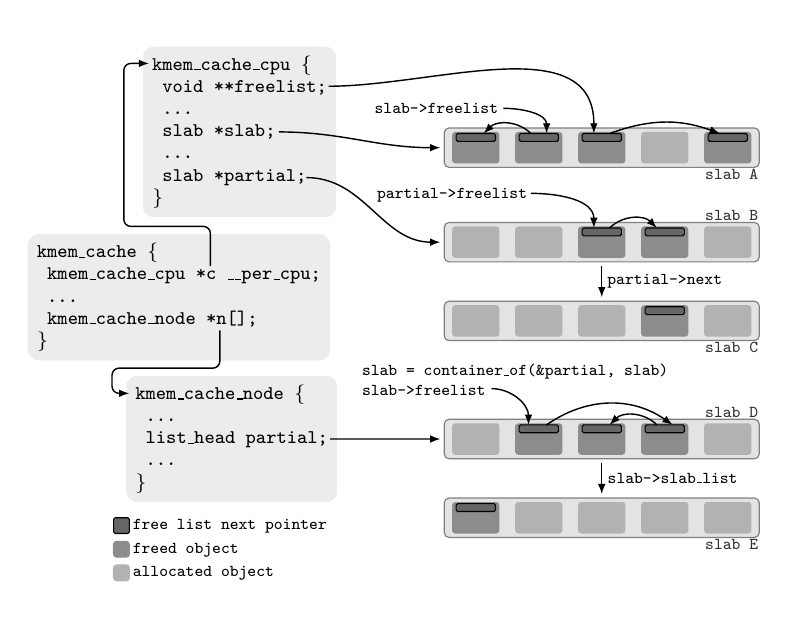
\begin{tikzpicture}

    \tikzstyle{slab}+=[
        rounded corners,
        rounded corners=0.6mm,
        line width = 0.15mm,
        gray,
        draw,
        rectangle,
        minimum width = 4cm,
        minimum height = 0.5cm,
        fill = gray!22
    ]
    \tikzstyle{object}+=[
        rounded corners,
        rounded corners=0.4mm,
        line width = 0.15mm,
        rectangle,
        minimum width = 0.6cm,
        minimum height = 0.4cm
    ]
    \tikzstyle{ptr}+=[
        rounded corners,
        rounded corners = 0.2mm,
        fill = black!60,
    ]
    \tikzstyle{freeobject}+=[
        object,
        fill = gray!90,
        gray!90,
    ]
    \tikzstyle{allocobject}+=[
        object,
        fill = gray!60,
        gray!60,
    ]
    \tikzstyle{onlytext}+=[
        align = left,
        font = \ttfamily\fontsize{6.5}{7.2}\selectfont
    ]
    \tikzstyle{ctext}+=[
        font = \ttfamily\scriptsize,
        rounded corners,
        fill = gray!15,
        align = left
    ]
    \tikzstyle{arrow}+=[
        -{Latex[length=1.3mm]},
        rounded corners=0.9mm,
        line width = 0.18mm
    ]
    \tikzstyle{arrow_indirect}+=[
        arrow,
        dashed,
        dash pattern=on 1.5pt off 1.5pt
    ]

    % ----------------------------------------------------------------------------
    \coordinate(kmem_cache) at (-5.17, -0.1);
    \coordinate(kmem_cache_cpu) at (-4.4, 2);
    \coordinate(kmem_cache_node) at (-4.5, -1.9);

    % ----------------------------------------------------------------------------
    \node[ctext] at (kmem_cache) {kmem\_cache \{\\\ kmem\_cache\_cpu *c \_\_per\_cpu;\\\ ...\\\ kmem\_cache\_node *n[];\\\}};
    \node[ctext] at (kmem_cache_cpu) {kmem\_cache\_cpu \{\\\ void **freelist;\\\ ...\\\ slab *slab;\\\ ...\\\ slab *partial;\\\}};
    \node[ctext] at (kmem_cache_node) {kmem\_cache\_node \{\\\ ...\\\ list\_head partial;\\\ ...\\\}};

    % ----------------------------------------------------------------------------
    \draw[arrow] ([shift=(kmem_cache)]0.4, 0.4) -- ([shift=(kmem_cache)]0.4, 0.9) -- ([shift=(kmem_cache)]-0.7, 0.9) --  ([shift=(kmem_cache_cpu)]-1.47, 0.87) -- ([shift=(kmem_cache_cpu)]-1.15, 0.87);
    \draw[arrow] ([shift=(kmem_cache)]0.52, -0.42) -- ([shift=(kmem_cache)]0.52, -0.9) -- ([shift=(kmem_cache)]-0.85, -0.9) -- ([shift=(kmem_cache_node)]-1.52, 0.58) -- ([shift=(kmem_cache_node)]-1.3, 0.58);

    % ----------------------------------------------------------------------------
    \coordinate(slab_start) at (0.2, -0.3);

    \coordinate(slab1) at ([shift=(slab_start)]0, 2.1);
    \coordinate(obj11) at ([shift=(slab1)]1.6, 0);
    \coordinate(obj12) at ([shift=(slab1)]0.8, 0);
    \coordinate(obj13) at ([shift=(slab1)]0, 0);
    \coordinate(obj14) at ([shift=(slab1)]-0.8, 0);
    \coordinate(obj15) at ([shift=(slab1)]-1.6, 0);

    \coordinate(slab2) at ([shift=(slab_start)]0, 0.9);
    \coordinate(obj21) at ([shift=(slab2)]1.6, 0);
    \coordinate(obj22) at ([shift=(slab2)]0.8, 0);
    \coordinate(obj23) at ([shift=(slab2)]0, 0);
    \coordinate(obj24) at ([shift=(slab2)]-0.8, 0);
    \coordinate(obj25) at ([shift=(slab2)]-1.6, 0);

    \coordinate(slab3) at ([shift=(slab_start)]0, -0.1);
    \coordinate(obj31) at ([shift=(slab3)]1.6, 0);
    \coordinate(obj32) at ([shift=(slab3)]0.8, 0);
    \coordinate(obj33) at ([shift=(slab3)]0, 0);
    \coordinate(obj34) at ([shift=(slab3)]-0.8, 0);
    \coordinate(obj35) at ([shift=(slab3)]-1.6, 0);

    \coordinate(slab4) at ([shift=(slab_start)]0, -1.6);
    \coordinate(obj41) at ([shift=(slab4)]1.6, 0);
    \coordinate(obj42) at ([shift=(slab4)]0.8, 0);
    \coordinate(obj43) at ([shift=(slab4)]0, 0);
    \coordinate(obj44) at ([shift=(slab4)]-0.8, 0);
    \coordinate(obj45) at ([shift=(slab4)]-1.6, 0);

    \coordinate(slab5) at ([shift=(slab_start)]0, -2.6);
    \coordinate(obj51) at ([shift=(slab5)]1.6, 0);
    \coordinate(obj52) at ([shift=(slab5)]0.8, 0);
    \coordinate(obj53) at ([shift=(slab5)]0, 0);
    \coordinate(obj54) at ([shift=(slab5)]-0.8, 0);
    \coordinate(obj55) at ([shift=(slab5)]-1.6, 0);

    % ----------------------------------------------------------------------------
    \coordinate(slab_freelist) at ([shift=(obj15)]-0.5, 0.5);
    \coordinate(partial_freelist) at ([shift=(obj25)]-0.3, 0.6);
    \coordinate(slab_container_of) at ([shift=(obj45)]0.5, 0.75);

    % ----------------------------------------------------------------------------
    \node[slab] at (slab1) {};
    \node[onlytext, black!80] at ([shift=(slab1)]1.65, -0.34) {slab A};
    \node[freeobject] at (obj11) {};
    \draw[ptr] ([shift=(obj11)]-0.25, 0.08) rectangle ++(0.5,0.1);
    \node[allocobject] at (obj12) {};
    \node[freeobject] at (obj13) {};
    \draw[ptr] ([shift=(obj13)]-0.25, 0.08) rectangle ++(0.5,0.1);
    \node[freeobject] at (obj14) {};
    \draw[ptr] ([shift=(obj14)]-0.25, 0.08) rectangle ++(0.5,0.1);
    \node[freeobject] at (obj15) {};
    \draw[ptr] ([shift=(obj15)]-0.25, 0.08) rectangle ++(0.5,0.1);

    \node[slab] at (slab2) {};
    \node[onlytext, black!80] at ([shift=(slab2)]1.65, 0.34) {slab B};
    \node[allocobject] at (obj21) {};
    \node[freeobject] at (obj22) {};
    \draw[ptr] ([shift=(obj22)]-0.25, 0.08) rectangle ++(0.5,0.1);
    \node[freeobject] at (obj23) {};
    \draw[ptr] ([shift=(obj23)]-0.25, 0.08) rectangle ++(0.5,0.1);
    \node[allocobject] at (obj24) {};
    \node[allocobject] at (obj25) {};

    \node[slab] at (slab3) {};
    \node[onlytext, black!80] at ([shift=(slab3)]1.65, -0.34) {slab C};
    \node[allocobject] at (obj31) {};
    \node[freeobject] at (obj32) {};
    \draw[ptr] ([shift=(obj32)]-0.25, 0.08) rectangle ++(0.5,0.1);
    \node[allocobject] at (obj33) {};
    \node[allocobject] at (obj34) {};
    \node[allocobject] at (obj35) {};

    \node[slab] at (slab4) {};
    \node[onlytext, black!80] at ([shift=(slab4)]1.65, 0.34) {slab D};
    \node[allocobject] at (obj41) {};
    \node[freeobject] at (obj42) {};
    \draw[ptr] ([shift=(obj42)]-0.25, 0.08) rectangle ++(0.5,0.1);
    \node[freeobject] at (obj43) {};
    \draw[ptr] ([shift=(obj43)]-0.25, 0.08) rectangle ++(0.5,0.1);
    \node[freeobject] at (obj44) {};
    \draw[ptr] ([shift=(obj44)]-0.25, 0.08) rectangle ++(0.5,0.1);
    \node[allocobject] at (obj45) {};

    \node[slab] at (slab5) {};
    \node[onlytext, black!80] at ([shift=(slab5)]1.65, -0.34) {slab E};
    \node[allocobject] at (obj51) {};
    \node[allocobject] at (obj52) {};
    \node[allocobject] at (obj53) {};
    \node[allocobject] at (obj54) {};
    \node[freeobject] at (obj55) {};
    \draw[ptr] ([shift=(obj55)]-0.25, 0.08) rectangle ++(0.5,0.1);

    % ----------------------------------------------------------------------------
    \draw[arrow] ([shift=(kmem_cache_cpu)]0.5, 0) to [out=0, in=180] ([shift=(slab1)]-2.05, 0);
    \draw[arrow] ([shift=(kmem_cache_cpu)]0.85, -0.58) to [out=0, in=180] ([shift=(slab2)]-2.05, 0);
    \draw[arrow] ([shift=(slab2)]0, -0.3) to [out=270, in=90] ([shift=(slab3)]0, 0.3);
    \node[onlytext] at ([shift=(slab2)]0.8, -0.5) {partial->next};
    \draw[arrow] ([shift=(kmem_cache_node)]1.25, 0) to [out=0, in=180] ([shift=(slab4)]-2.05, 0);
    \draw[arrow] ([shift=(slab4)]0, -0.3) to [out=270, in=90] ([shift=(slab5)]0, 0.3);
    \node[onlytext] at ([shift=(slab4)]0.9, -0.5) {slab->slab\_list};

    \draw[arrow] ([shift=(kmem_cache_cpu)]1.13, 0.58) to [out=0, in=90] ([shift=(obj13)]-0.1, 0.18);
    \draw[arrow, bend left=20] ([shift=(obj13)]0.1, 0.18) to ([shift=(obj11)]-0.1, 0.18);
    \draw[arrow, bend left=-45] ([shift=(obj14)]-0.1, 0.18) to ([shift=(obj15)]0.1, 0.18);

    \draw[arrow, bend left=45] ([shift=(obj23)]0.1, 0.18) to ([shift=(obj22)]-0.1, 0.18);

    \draw[arrow, bend left=35] ([shift=(obj44)]0.1, 0.18) to ([shift=(obj42)]0.1, 0.18);
    \draw[arrow, bend left=-45] ([shift=(obj42)]-0.1, 0.18) to ([shift=(obj43)]0.1, 0.18);

    % ----------------------------------------------------------------------------
    \node[onlytext] at (slab_freelist) {slab->freelist};
    \draw[arrow] ([shift=(slab_freelist)]0.85, 0) to [out=0, in=90] ([shift=(obj14)]0.1, 0.18);
    \node[onlytext] at (partial_freelist) {partial->freelist};
    \draw[arrow] ([shift=(partial_freelist)]1, 0.02) to [out=0, in=90] ([shift=(obj23)]-0.1, 0.18);
    \node[onlytext] at (slab_container_of) {slab = container\_of(\&partial, slab)\\slab->freelist};
    \draw[arrow] ([shift=(slab_container_of)]-0.3, -0.11) to [out=0, in=90] ([shift=(obj44)]-0.13, 0.18);

    % ----------------------------------------------------------------------------
    \coordinate(legend) at (-6,-3.1);
    \draw[ptr] (legend) rectangle ++(0.2,0.2);
    \node[onlytext, anchor=west] at ([shift=(legend)]0.12, 0.09) {free list next pointer};
    \draw[freeobject] ([shift=(legend)]0, -0.3) rectangle ++(0.2,0.2);
    \node[onlytext, anchor=west] at ([shift=(legend)]0.12, -0.21) {freed object};
    \draw[allocobject] ([shift=(legend)]0, -0.6) {rectangle ++(0.2,0.2)};
    \node[onlytext, anchor=west] at ([shift=(legend)]0.12, -0.51) {allocated object};

\end{tikzpicture}
\end{document}
